\section{ASCbase::Sitemap Class Reference}
\label{classASCbase_1_1Sitemap}\index{ASCbase::Sitemap@{ASCbase::Sitemap}}
{\tt \#include $<$Sitemap.H$>$}

Inheritance diagram for ASCbase::Sitemap::\begin{figure}[H]
\begin{center}
\leavevmode
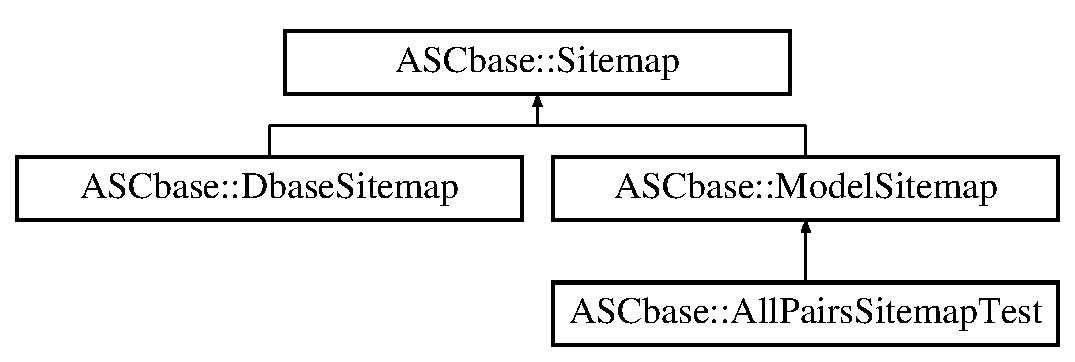
\includegraphics[height=3cm]{classASCbase_1_1Sitemap}
\end{center}
\end{figure}
\subsection*{Public Member Functions}
\begin{CompactItemize}
\item 
\bf{Sitemap} (const std::string path, const std::string struct\_\-id, const \bf{Base\-Parameters} \&args, const bool normalize=true, const bool load\_\-hbond\_\-surfaces=false, const bool hydrophobic\_\-query=false, const verbose\_\-level\_\-t verbosity=VERBOSE\_\-SILENT)\label{classASCbase_1_1Sitemap_50c5a65ec5c3b1e196466431ab71637a}

\begin{CompactList}\small\item\em Read/load a sitemap. \item\end{CompactList}\item 
\bf{Sitemap} (const \bf{Gen\-Points\-Parameters} \&usr\_\-args)\label{classASCbase_1_1Sitemap_fc5a254b492d94440c55970ef63386f2}

\begin{CompactList}\small\item\em First step in creating a sitemap. \item\end{CompactList}\item 
virtual \bf{$\sim$Sitemap} ()\label{classASCbase_1_1Sitemap_efd8a95708982d72800caf7f69073700}

\begin{CompactList}\small\item\em Typical cleanup of dynamic mem. \item\end{CompactList}\item 
bool \bf{fail} () const 
\begin{CompactList}\small\item\em Check if class is viable. \item\end{CompactList}\item 
bool \bf{write\_\-files} (const std::string struct\_\-id, const std::string path)\label{classASCbase_1_1Sitemap_88720d257d371462b7fc1b8c797aa697}

\begin{CompactList}\small\item\em Write the three sitemap files. \item\end{CompactList}\item 
bool \bf{has\_\-enough\_\-points} ()
\item 
std::string \bf{atoms\_\-file\_\-name} () const \label{classASCbase_1_1Sitemap_aaf9fd841e8f5a03b2b7b756240bbe82}

\begin{CompactList}\small\item\em Get the filename of the PDB structure used to generate the sitemap. \item\end{CompactList}\item 
std::string \bf{ligand\_\-file\_\-name} () const \label{classASCbase_1_1Sitemap_cb41876f6caf930dbfd134532ba02a0c}

\begin{CompactList}\small\item\em Get the filename of the mol2 ligand used to generate the sitemap. \item\end{CompactList}\item 
const \bf{Sitemap\-Atoms\-File} \& \textbf{interacting\_\-atoms} () const \label{classASCbase_1_1Sitemap_8cef15e389674f18b95f808397f30163}

\item 
\bf{Sitemap\-Atoms\-File} \& \textbf{interacting\_\-atoms} ()\label{classASCbase_1_1Sitemap_49015f2e7b31c7f19a0a47abc9af3db2}

\item 
const \bf{PDBStructure} \& \textbf{bind\_\-site\_\-atoms} () const \label{classASCbase_1_1Sitemap_e56f41b7103116460be52ca6be7f2549}

\item 
\bf{PDBStructure} \& \textbf{bind\_\-site\_\-atoms} ()\label{classASCbase_1_1Sitemap_7c01c7079e267cf260d1c7e255ae6b6f}

\item 
const \bf{Sitemap\-Points\-File} \& \textbf{sitemap\_\-points} () const \label{classASCbase_1_1Sitemap_5bdd019adc94558d333e1b988a574b32}

\item 
interact\_\-pts\_\-vci \textbf{interact\_\-pts\_\-beg} () const \label{classASCbase_1_1Sitemap_a7ad7e74e6ef0cdfb3e8e487e2db6200}

\item 
interact\_\-pts\_\-vci \textbf{interact\_\-pts\_\-end} () const \label{classASCbase_1_1Sitemap_fe90bda50b24ac3ecfa92df9d698b7d1}

\item 
void \textbf{transform\_\-interact\_\-pts} (my\_\-float\_\-t $\ast$R, my\_\-float\_\-t $\ast$T)\label{classASCbase_1_1Sitemap_dbd2a6cb931e9a427fa8543216600632}

\item 
void \textbf{revert\_\-interact\_\-pts} ()\label{classASCbase_1_1Sitemap_ec8a4a45362b46f0fd2f25db0876f488}

\item 
void \textbf{interact\_\-pts\_\-centroid\_\-3D} (my\_\-float\_\-t $\ast$C)\label{classASCbase_1_1Sitemap_f6ea975d404459e84b1283b3d011434f}

\item 
\bf{Hbond\-Points} \& \bf{hbond\_\-points} ()\label{classASCbase_1_1Sitemap_007b084d4422bb7a72bdd63e309985ce}

\begin{CompactList}\small\item\em Get a reference to the sitemap hbond points. \item\end{CompactList}\item 
const \bf{Hbond\-Points} \& \bf{hbond\_\-points} () const \label{classASCbase_1_1Sitemap_d985aeaf02eedb866b67eb389e62df52}

\begin{CompactList}\small\item\em Get a const reference to the sitemap hbond points. \item\end{CompactList}\item 
\bf{Hphob\-Points} \& \bf{hphob\_\-points} ()\label{classASCbase_1_1Sitemap_ac2a508a7cb5843d2450b4261de23b93}

\begin{CompactList}\small\item\em Get a reference to the sitemap hphob points. \item\end{CompactList}\item 
const \bf{Hphob\-Points} \& \bf{hphob\_\-points} () const \label{classASCbase_1_1Sitemap_0ee5530e8852f95876a978e8c284f88f}

\begin{CompactList}\small\item\em Get a const reference to the sitemap hphob points. \item\end{CompactList}\item 
size\_\-t \textbf{fit\_\-points\_\-size} () const \label{classASCbase_1_1Sitemap_88f86e7f2f8a1a69a6e34a1b6b942216}

\item 
const my\_\-float\_\-t $\ast$ \textbf{get\_\-norm\_\-moments} () const \label{classASCbase_1_1Sitemap_df498664611c91d15cf7234d8ef91dbc}

\item 
void \textbf{transform\_\-bind\_\-site\_\-res\_\-pos} (const my\_\-float\_\-t $\ast$R, const my\_\-float\_\-t $\ast$T)\label{classASCbase_1_1Sitemap_22aa833d2798ec1ecc85f29444a60dc2}

\item 
void \textbf{revert\_\-bind\_\-site\_\-res\_\-pos} ()\label{classASCbase_1_1Sitemap_2411adae66ef848c5bfe67d55c07e672}

\item 
const \bf{Bounding\-Volume} \& \textbf{bounding\_\-volume\_\-handle} () const \label{classASCbase_1_1Sitemap_3ba92f5ed263d28b96b29085c197abed}

\item 
const \bf{Bounding\-Volume} \& \textbf{site\_\-volume\_\-estimate\_\-handle} () const \label{classASCbase_1_1Sitemap_ad6269d1f92809bbf093a0c6f6c8442a}

\item 
void \textbf{revert} ()\label{classASCbase_1_1Sitemap_85a7198a79dd727691347e20c5ffffef}

\item 
my\_\-float\_\-t \bf{compute\_\-RMSD} () const 
\item 
void \bf{transform} (const my\_\-float\_\-t $\ast$R, const my\_\-float\_\-t $\ast$T)\label{classASCbase_1_1Sitemap_5dc7a050ffc9ae70c203cb31e41b4b77}

\begin{CompactList}\small\item\em Transform the objects that comprise the model of the binding site. \item\end{CompactList}\item 
void \bf{inverse\_\-transform} (const my\_\-float\_\-t $\ast$R, const my\_\-float\_\-t $\ast$T)
\item 
Hbond\-Surfaces$<$ \bf{hbond\_\-surface\_\-t} $>$ \& \textbf{hbond\_\-surfaces} () const \label{classASCbase_1_1Sitemap_9e75ff867b2874ad6365c5c67c27a941}

\item 
std::string \textbf{site\_\-path} () const \label{classASCbase_1_1Sitemap_25f76f5d2bfbce099424bce78913d77b}

\item 
std::string \textbf{get\_\-struct\_\-id} () const \label{classASCbase_1_1Sitemap_325a5ef0a4b1949fd1d7eb8622a91802}

\item 
void \bf{compute\_\-max\_\-feature\_\-values} (std::vector$<$ my\_\-float\_\-t $>$ $\ast$max\_\-feat\_\-vals) const 
\item 
my\_\-float\_\-t \bf{compute\_\-site\_\-vol\_\-intersect} (const \bf{Sitemap} \&other) const 
\end{CompactItemize}
\subsection*{Protected Member Functions}
\begin{CompactItemize}
\item 
void \textbf{set\_\-fail\_\-flag} (const bool val)\label{classASCbase_1_1Sitemap_e250f1412ec1750e343811d8582cd562}

\item 
bool \textbf{load\_\-volume} (std::string path, std::string struct\_\-id, std::string dbase\_\-sites, std::string vol\_\-tag, \bf{Bounding\-Volume} $\ast$$\ast$vol, geometry::sphere\_\-t $\ast$S=0)\label{classASCbase_1_1Sitemap_79a3b9c79bdd450b23932618525d67ae}

\end{CompactItemize}
\subsection*{Protected Attributes}
\begin{CompactItemize}
\item 
\bf{Hbond\-Points} $\ast$ \bf{hbond\_\-pts}\label{classASCbase_1_1Sitemap_dcd2dacc1cda6d35e9e477e38ab1af5b}

\begin{CompactList}\small\item\em Hydrophillic portion of sitemap. \item\end{CompactList}\item 
\bf{Hphob\-Points} $\ast$ \bf{hphob\_\-pts}\label{classASCbase_1_1Sitemap_89271f4fedad4a8435ff3f30e58bb7f7}

\begin{CompactList}\small\item\em Hydrophobic portion of sitemap. \item\end{CompactList}\item 
\bf{interact\_\-pts\_\-vec} \textbf{interact\_\-points}\label{classASCbase_1_1Sitemap_ff5f52340679a7c4c44521a8f7218324}

\item 
\bf{Bounding\-Volume} $\ast$ \bf{A\_\-site\_\-vol\_\-est}\label{classASCbase_1_1Sitemap_cb78a63c2111c987ecd011d1dd3d1ce0}

\begin{CompactList}\small\item\em Upper estimate of the site volume. \item\end{CompactList}\end{CompactItemize}
\subsection*{Private Member Functions}
\begin{CompactItemize}
\item 
void \bf{init} ()\label{classASCbase_1_1Sitemap_2c579b022413645a8ecbdc4317117563}

\begin{CompactList}\small\item\em Initialize class pointer variables to zero (NULL). \item\end{CompactList}\item 
bool \textbf{get\_\-user\_\-surf\_\-patches} (const std::string \&lig\_\-fname, const std::string \&scratch\_\-dir, const std::string \&sphere\_\-str, const std::string \&user\_\-vert\_\-fname)\label{classASCbase_1_1Sitemap_bc73bf05cc0b7795b178657d537ab7d9}

\item 
bool \textbf{get\_\-MSMS\_\-surf\_\-patches} (const std::string \&lig\_\-fname, const std::string \&scratch\_\-dir, const std::string \&sphere\_\-str, const std::string \&install\_\-dir, const bool include\_\-metals, const std::string \&msms\_\-binary, const std::vector$<$ std::string $>$ \&waters)\label{classASCbase_1_1Sitemap_a35e5cc0fa7e11df3b9f5f237a01ab5c}

\item 
bool \bf{get\_\-norm\_\-stats} (const std::string csv\_\-fname, const \bf{Base\-Parameters} \&args, bool hydrophobic\_\-query=false)\label{classASCbase_1_1Sitemap_d692fc3eae9705af5c3b5151a18aad82}

\begin{CompactList}\small\item\em Get the normalization stats for the given sitemap file. \item\end{CompactList}\item 
\bf{Bounding\-Volume} $\ast$ \bf{setup\_\-volume} (const std::string ligand\_\-fname, const my\_\-float\_\-t grid\_\-spacing, const std::string sphere\_\-str, const bool use\_\-union\_\-of\_\-balls)
\begin{CompactList}\small\item\em Setup the sitemap volume. \item\end{CompactList}\item 
void \textbf{get\_\-prot\_\-interact\_\-atoms} (const \bf{PDBStructure} $\ast$prot, \bf{Bounding\-Volume} $\ast$site\_\-vol, std::vector$<$ atom\_\-vci $>$ $\ast$bind\_\-atoms, std::vector$<$ atom\_\-vci $>$ $\ast$rad\_\-atoms, interact\_\-atoms\_\-vec $\ast$hbond\_\-atoms, interact\_\-atoms\_\-vec $\ast$hphob\_\-atoms, hphob\_\-triad\_\-vec $\ast$hphob\_\-triads, const int min\_\-chain\_\-size)\label{classASCbase_1_1Sitemap_b38affd80a93bb4445f22c732b79e8cb}

\item 
void \bf{find\_\-binding\_\-site\_\-hbonds} (const \bf{Gen\-Points\-Parameters::hbond\_\-method\_\-t} hbond\_\-density, const std::string params\_\-dir, const std::vector$<$ std::string $>$ \&waters, \bf{Bounding\-Volume} $\ast$site\_\-vol, const interact\_\-atoms\_\-vec \&hbond\_\-atoms, std::vector$<$ atom\_\-vci $>$ $\ast$bind\_\-atoms, std::vector$<$ atom\_\-vci $>$ $\ast$rad\_\-atoms)
\item 
bool \bf{find\_\-binding\_\-site\_\-metals} ()\label{classASCbase_1_1Sitemap_4fcf9aa2c2a4afcf1d21bd3038434d7d}

\begin{CompactList}\small\item\em Calculate the template points for all metal atoms in the binding site. \item\end{CompactList}\item 
bool \bf{find\_\-binding\_\-site\_\-hphobs} (const \bf{Gen\-Points\-Parameters::hphob\_\-method\_\-t} hphob\_\-method, const my\_\-float\_\-t cluster\_\-diameter, const interact\_\-atoms\_\-vec \&hphob\_\-atoms, const hphob\_\-triad\_\-vec \&hphob\_\-triads, const std::vector$<$ atom\_\-vci $>$ \&bind\_\-atoms, \bf{Bounding\-Volume} $\ast$site\_\-vol, const sphere\_\-sample\_\-level\_\-t sample\_\-level=DISCRETE\_\-SPHERE\_\-LEVEL\_\-TWO)
\item 
void \bf{write\_\-feature\_\-scales} (std::ostream \&out)\label{classASCbase_1_1Sitemap_1596bc4cf18ba4f6709a67f3e30437cb}

\begin{CompactList}\small\item\em Write out the largest value possible for each feature. \item\end{CompactList}\item 
void \textbf{clean\_\-up\_\-string} (std::string \&S)\label{classASCbase_1_1Sitemap_0894845a3e513c909d694bbd0fdcaba3}

\item 
void \textbf{build\_\-points\_\-header} (const \bf{Gen\-Points\-Parameters} \&args)\label{classASCbase_1_1Sitemap_2f3a6d65a3e920903d9d4869c168510d}

\item 
bool \textbf{gen\_\-lig\_\-box} (const std::string fname, my\_\-float\_\-t $\ast$corners)\label{classASCbase_1_1Sitemap_583a1a32407f665be875abee7e6744d2}

\item 
void \textbf{get\_\-site\_\-volume\_\-estimate} (hbond\_\-fit\_\-pt\_\-vci hbond\_\-pts\_\-beg, hbond\_\-fit\_\-pt\_\-vci hbond\_\-pts\_\-end, hphob\_\-point\_\-lci hphob\_\-points\_\-beg, hphob\_\-point\_\-lci hphob\_\-points\_\-end, size\_\-t npts, my\_\-float\_\-t vol\_\-est\_\-tol)\label{classASCbase_1_1Sitemap_6fc2cf350f7c9dbe24ef402196d601d5}

\item 
bool \textbf{load\_\-ligand} (const std::string \&fname, \bf{Coord\-File} $\ast$$\ast$lig)\label{classASCbase_1_1Sitemap_4c1be8761d14961907869cd902292581}

\item 
bool \textbf{get\_\-prot\_\-atom\_\-close\_\-to\_\-ligand} (const std::string ligand\_\-fname, std::vector$<$ atom\_\-vci $>$ \&bind\_\-atoms, atom\_\-vci $\ast$close\_\-atom)\label{classASCbase_1_1Sitemap_d896226d048c6c0f9347bee48b938f86}

\end{CompactItemize}
\subsection*{Private Attributes}
\begin{CompactItemize}
\item 
verbose\_\-level\_\-t \textbf{verbose}\label{classASCbase_1_1Sitemap_b030f50473b6d8670e571d51003f424d}

\item 
\bf{Bounding\-Volume} $\ast$ \textbf{A\_\-site\_\-vol}\label{classASCbase_1_1Sitemap_6990d012cf2b73d02b1a953df6bea5b9}

\item 
\bf{Sitemap\-Atoms\-File} $\ast$ \bf{A\_\-site\_\-atoms}\label{classASCbase_1_1Sitemap_aacf141914798bdd7861687e432628f8}

\begin{CompactList}\small\item\em Atoms from residues near the binding site. \item\end{CompactList}\item 
\bf{PDBStructure} $\ast$ \textbf{A\_\-bind\_\-site\_\-res}\label{classASCbase_1_1Sitemap_2a52e689037b97d6a36e93507c7883ea}

\item 
\bf{Sitemap\-Points\-File} $\ast$ \textbf{points}\label{classASCbase_1_1Sitemap_0d487acfbafbcd354984bc9ee12d4f18}

\item 
\bf{PDBStructure} $\ast$ \textbf{prot\_\-atoms}\label{classASCbase_1_1Sitemap_d14802c86d41cb3aebbad567ab57cde0}

\item 
atom\_\-map\_\-t \textbf{interact\_\-atoms}\label{classASCbase_1_1Sitemap_104c9c8b0dc2d1c8239e24ff9ae16d30}

\item 
my\_\-float\_\-t \textbf{A\_\-norm\_\-moments} [2]\label{classASCbase_1_1Sitemap_3b31d195203a3e0b86a9b4e42f29aefe}

\item 
my\_\-float\_\-t \textbf{A\_\-hphob\_\-norm\_\-moments} [2]\label{classASCbase_1_1Sitemap_710b85700b6359566aa94d1cb3b23ad0}

\item 
Hbond\-Surfaces$<$ \bf{hbond\_\-surface\_\-t} $>$ $\ast$ \textbf{A\_\-hbond\_\-surfaces}\label{classASCbase_1_1Sitemap_746f37a116532d40ebfb917405f79f56}

\item 
\bf{Simple\-Trimesh} $\ast$ \textbf{old\_\-binding\_\-site\_\-mesh}\label{classASCbase_1_1Sitemap_67d0c9dd4ca44665912f7927effd2478}

\item 
geometry::sphere\_\-t \bf{A\_\-site\_\-vol\_\-est\_\-as\_\-sphere}\label{classASCbase_1_1Sitemap_d868aaadd592ee46383e0ab2e9cc9350}

\begin{CompactList}\small\item\em I don't have the time to compute the intersection of the different bounding volume classes -- use this instead. \item\end{CompactList}\item 
std::string \bf{A\_\-site\_\-path}\label{classASCbase_1_1Sitemap_f9703909778c885c912a1415910f988f}

\begin{CompactList}\small\item\em Directory holding the sitemap. \item\end{CompactList}\item 
std::string \bf{A\_\-struct\_\-id}\label{classASCbase_1_1Sitemap_1355b26f18d6bd22405fc2ed95543b68}

\begin{CompactList}\small\item\em Structure ID of the site map. \item\end{CompactList}\item 
std::string \bf{A\_\-dbase\_\-ligs}\label{classASCbase_1_1Sitemap_f759f963ef40e2d5b8bfe0805f70e2f8}

\begin{CompactList}\small\item\em Directory holding dbase ligands. \item\end{CompactList}\item 
std::string \bf{A\_\-lig\_\-fname}\label{classASCbase_1_1Sitemap_8687cc1a0a4f3c900d40bc3b3ba7b4bb}

\begin{CompactList}\small\item\em Name of the ligand file. \item\end{CompactList}\item 
std::string \bf{A\_\-atoms\_\-fname}\label{classASCbase_1_1Sitemap_22af7b3e2f83f482711f96fd2b8036fb}

\begin{CompactList}\small\item\em Name of the sitemap atoms file. \item\end{CompactList}\item 
bool \textbf{A\_\-include\_\-metals}\label{classASCbase_1_1Sitemap_085592f9e6ab4a46b1717d17e15f3590}

\item 
bool \textbf{A\_\-MSMS\_\-surf}\label{classASCbase_1_1Sitemap_cc87543764821d5965c02426e3b621c0}

\item 
bool \textbf{A\_\-user\_\-surf}\label{classASCbase_1_1Sitemap_8a9754cb39062045c87758860244e132}

\item 
my\_\-float\_\-t \bf{A\_\-probe\_\-radius}\label{classASCbase_1_1Sitemap_7474a2670e5f74e20594a2add689f8d5}

\begin{CompactList}\small\item\em Probe radius for MSMS. \item\end{CompactList}\item 
my\_\-float\_\-t \bf{A\_\-num\_\-pts\_\-per\_\-area}\label{classASCbase_1_1Sitemap_f9dbc37200a6d1841ea366760f8d0837}

\begin{CompactList}\small\item\em Number of points per (A)$^\wedge$2. \item\end{CompactList}\item 
int \textbf{A\_\-min\_\-res\_\-per\_\-chain}\label{classASCbase_1_1Sitemap_ca99b08072b44f7f26cd714417333b44}

\item 
bool \textbf{A\_\-fail}\label{classASCbase_1_1Sitemap_960c9c48a78c77be9eae68071e34e987}

\end{CompactItemize}
\subsection*{Static Private Attributes}
\begin{CompactItemize}
\item 
static const int \textbf{MIN\_\-NUMBER\_\-POINTS\_\-\_\-POLAR\_\-SITE} = 20\label{classASCbase_1_1Sitemap_693e69f1d3787c869c7510692bcd0e91}

\item 
static const int \textbf{MIN\_\-NUMBER\_\-POINTS\_\-\_\-HPHOB\_\-SITE} = 30\label{classASCbase_1_1Sitemap_fd1fc07d472e969eb867e04bbe1170e6}

\item 
static const my\_\-float\_\-t \textbf{TOLERANCE} = 2.0\label{classASCbase_1_1Sitemap_872ebaa52aa3fdf3501804dd35077f84}

\item 
static const my\_\-float\_\-t \bf{MAXRADDIST}\label{classASCbase_1_1Sitemap_5eeb7fdc83ae79798995a668a58b42e1}

\begin{CompactList}\small\item\em Max rad file dist? \item\end{CompactList}\item 
static const my\_\-float\_\-t \bf{MAXBINDDIST}\label{classASCbase_1_1Sitemap_7cf5dd107e339908dc8ca026eba23360}

\begin{CompactList}\small\item\em Max interaction with binding site dist. \item\end{CompactList}\item 
static const std::string \bf{A\_\-fname} = \char`\"{}Sitemap.C\char`\"{}\label{classASCbase_1_1Sitemap_b28ac13500885c7b52d35446d3fa89de}

\begin{CompactList}\small\item\em Name of source file. \item\end{CompactList}\end{CompactItemize}


\subsection{Detailed Description}
Both generates and loads sitemaps. Kinda glues together the different parts in an ad hoc manner. This works, but the interface is quite clunky. 



\subsection{Member Function Documentation}
\index{ASCbase::Sitemap@{ASCbase::Sitemap}!compute_max_feature_values@{compute\_\-max\_\-feature\_\-values}}
\index{compute_max_feature_values@{compute\_\-max\_\-feature\_\-values}!ASCbase::Sitemap@{ASCbase::Sitemap}}
\subsubsection{\setlength{\rightskip}{0pt plus 5cm}void Sitemap::compute\_\-max\_\-feature\_\-values (std::vector$<$ my\_\-float\_\-t $>$ $\ast$ {\em max\_\-feat\_\-vals}) const}\label{classASCbase_1_1Sitemap_2fc4a9ede3730c0cd6fdadc97f00864b}


Compute the maximum value for each feature and store in the given vector \index{ASCbase::Sitemap@{ASCbase::Sitemap}!compute_RMSD@{compute\_\-RMSD}}
\index{compute_RMSD@{compute\_\-RMSD}!ASCbase::Sitemap@{ASCbase::Sitemap}}
\subsubsection{\setlength{\rightskip}{0pt plus 5cm}my\_\-float\_\-t ASCbase::Sitemap::compute\_\-RMSD () const\hspace{0.3cm}{\tt  [inline]}}\label{classASCbase_1_1Sitemap_81fe70b16f0e030e8c20923fc2e66a49}


Compute the root mean squared deviation (RMSD) between the current and orignial positions of the hydrogen bonding and hydrophobic points \index{ASCbase::Sitemap@{ASCbase::Sitemap}!compute_site_vol_intersect@{compute\_\-site\_\-vol\_\-intersect}}
\index{compute_site_vol_intersect@{compute\_\-site\_\-vol\_\-intersect}!ASCbase::Sitemap@{ASCbase::Sitemap}}
\subsubsection{\setlength{\rightskip}{0pt plus 5cm}my\_\-float\_\-t Sitemap::compute\_\-site\_\-vol\_\-intersect (const \bf{Sitemap} \& {\em other}) const}\label{classASCbase_1_1Sitemap_8865b700374d55d3e7b4d6c4cd489f60}


Compute the fraction of the volume of this site's volume estimate that is inside the other site's volume estimate \index{ASCbase::Sitemap@{ASCbase::Sitemap}!fail@{fail}}
\index{fail@{fail}!ASCbase::Sitemap@{ASCbase::Sitemap}}
\subsubsection{\setlength{\rightskip}{0pt plus 5cm}bool ASCbase::Sitemap::fail () const\hspace{0.3cm}{\tt  [inline]}}\label{classASCbase_1_1Sitemap_1a15e9045f766ba8e80f6411513de6ac}


Check if class is viable. 

\begin{Desc}
\item[Returns:]False if no fatal errors have occured, else true \end{Desc}
\index{ASCbase::Sitemap@{ASCbase::Sitemap}!find_binding_site_hbonds@{find\_\-binding\_\-site\_\-hbonds}}
\index{find_binding_site_hbonds@{find\_\-binding\_\-site\_\-hbonds}!ASCbase::Sitemap@{ASCbase::Sitemap}}
\subsubsection{\setlength{\rightskip}{0pt plus 5cm}void Sitemap::find\_\-binding\_\-site\_\-hbonds (const \bf{Gen\-Points\-Parameters::hbond\_\-method\_\-t} {\em hbond\_\-density}, const std::string {\em params\_\-dir}, const std::vector$<$ std::string $>$ \& {\em waters}, \bf{Bounding\-Volume} $\ast$ {\em site\_\-vol}, const interact\_\-atoms\_\-vec \& {\em hbond\_\-atoms}, std::vector$<$ atom\_\-vci $>$ $\ast$ {\em bind\_\-atoms}, std::vector$<$ atom\_\-vci $>$ $\ast$ {\em rad\_\-atoms})\hspace{0.3cm}{\tt  [private]}}\label{classASCbase_1_1Sitemap_1c89cc76612ae6e252b459b4bf62bc13}


\begin{Desc}
\item[Parameters:]
\begin{description}
\item[{\em hbond\_\-density}]Density to discretely sample hydrogen bonding volume \item[{\em params\_\-dir}]Directory holding the hbond point sampling files \item[{\em site\_\-vol}]Pointer to the sitemap volume \item[{\em include\_\-waters}]True implies include all water molecules in the protein structure as \char`\"{}part of the protein\char`\"{}. \item[{\em include\_\-metals}]True implies include all metal atoms in the the protein structure as \char`\"{}part of the protein\char`\"{}. \item[{\em rad\_\-atoms}]Pointer to vector to hold rad atoms. \end{description}
\end{Desc}
\index{ASCbase::Sitemap@{ASCbase::Sitemap}!find_binding_site_hphobs@{find\_\-binding\_\-site\_\-hphobs}}
\index{find_binding_site_hphobs@{find\_\-binding\_\-site\_\-hphobs}!ASCbase::Sitemap@{ASCbase::Sitemap}}
\subsubsection{\setlength{\rightskip}{0pt plus 5cm}bool Sitemap::find\_\-binding\_\-site\_\-hphobs (const \bf{Gen\-Points\-Parameters::hphob\_\-method\_\-t} {\em hphob\_\-method}, const my\_\-float\_\-t {\em cluster\_\-diameter}, const interact\_\-atoms\_\-vec \& {\em hphob\_\-atoms}, const hphob\_\-triad\_\-vec \& {\em hphob\_\-triads}, const std::vector$<$ atom\_\-vci $>$ \& {\em bind\_\-atoms}, \bf{Bounding\-Volume} $\ast$ {\em site\_\-vol}, const sphere\_\-sample\_\-level\_\-t {\em sample\_\-level} = {\tt DISCRETE\_\-SPHERE\_\-LEVEL\_\-TWO})\hspace{0.3cm}{\tt  [private]}}\label{classASCbase_1_1Sitemap_955ee3f2bcb9a0853c49c98f9664310b}


\begin{Desc}
\item[Parameters:]
\begin{description}
\item[{\em hphob\_\-method}]which hydrophobic model/method to use \item[{\em cluster\_\-diameter}]The maximum cluster diameter for complete link clustering of hphob points. \item[{\em rad\_\-atoms}]Reference to the rad atoms (returned from hbonds method) \end{description}
\end{Desc}
\begin{Desc}
\item[Returns:]!fail() \end{Desc}
\index{ASCbase::Sitemap@{ASCbase::Sitemap}!has_enough_points@{has\_\-enough\_\-points}}
\index{has_enough_points@{has\_\-enough\_\-points}!ASCbase::Sitemap@{ASCbase::Sitemap}}
\subsubsection{\setlength{\rightskip}{0pt plus 5cm}bool Sitemap::has\_\-enough\_\-points ()}\label{classASCbase_1_1Sitemap_e9d2433452ba04908e7ef43cbe7d8c3c}


Determine if the site map has enough points given the current implementation of the site maps, alignment method, and alignment techniques scoring \index{ASCbase::Sitemap@{ASCbase::Sitemap}!inverse_transform@{inverse\_\-transform}}
\index{inverse_transform@{inverse\_\-transform}!ASCbase::Sitemap@{ASCbase::Sitemap}}
\subsubsection{\setlength{\rightskip}{0pt plus 5cm}void ASCbase::Sitemap::inverse\_\-transform (const my\_\-float\_\-t $\ast$ {\em R}, const my\_\-float\_\-t $\ast$ {\em T})\hspace{0.3cm}{\tt  [inline]}}\label{classASCbase_1_1Sitemap_9923d897faab8e6b015908311241ac3a}


Transform the objects that comprise the model of the binding site using the inverse of the transform defined by R \& T \index{ASCbase::Sitemap@{ASCbase::Sitemap}!setup_volume@{setup\_\-volume}}
\index{setup_volume@{setup\_\-volume}!ASCbase::Sitemap@{ASCbase::Sitemap}}
\subsubsection{\setlength{\rightskip}{0pt plus 5cm}\bf{Bounding\-Volume} $\ast$ Sitemap::setup\_\-volume (const std::string {\em ligand\_\-fname}, const my\_\-float\_\-t {\em grid\_\-spacing}, const std::string {\em sphere\_\-str}, const bool {\em use\_\-union\_\-of\_\-balls})\hspace{0.3cm}{\tt  [private]}}\label{classASCbase_1_1Sitemap_dbc5be7e837523050ebf38da9fca1d1f}


Setup the sitemap volume. 

\begin{Desc}
\item[Parameters:]
\begin{description}
\item[{\em ligand\_\-fname}]Path to the ligand to define the binding site volume \item[{\em grid\_\-spacing}]The rectuangular grid sampling distance \item[{\em sphere\_\-str}]Sphere as center and radius in a string \item[{\em use\_\-union\_\-of\_\-balls}]If a ligand is given and use\_\-union\_\-of\_\-balls is true, take the union of balls (1 centered at each ligand atom) as the volume estimate and not the ligand bounding box. \end{description}
\end{Desc}
\begin{Desc}
\item[Returns:]Pointer to the volume object or NULL if an error occured \end{Desc}


The documentation for this class was generated from the following files:\begin{CompactItemize}
\item 
Sitemap.H\item 
Sitemap.C\end{CompactItemize}
